%!TEX root = ../mieic.tex


\chapter{Methodologies}
\label{chap:chap4}

\section*{}

In this chapter, further details about the methodologies used in the developed prototype, as well as in the the validation process, will be explored.

The development process will be compared to the previous expectations of the outcome of the planned prototype.

By this point, the validation of the prototype will be analysed, by explaining the performed user tests, as well the analysis of the results.


\section{Prototype} % (fold)
\label{sec:prototype}

  \subsection{Main Features} % (fold)
    \label{sub:main_features}
    
    The main features of RAMA's Spotify Application are: visualization of a map of a network of connected artists; edit the graph (expand and new map functions, as well as with the depth and branching parameters); Tags overlay and music artist info.

    \subsubsection{Visulization of the Artist Map} % (fold)
      \label{ssub:visualization}
    
      The application automatically draws the map with the current playing artist as the main node, as seen in Figure~\ref{fig:graph_rootnode}.

      \begin{figure}[tb]
        \begin{center}
          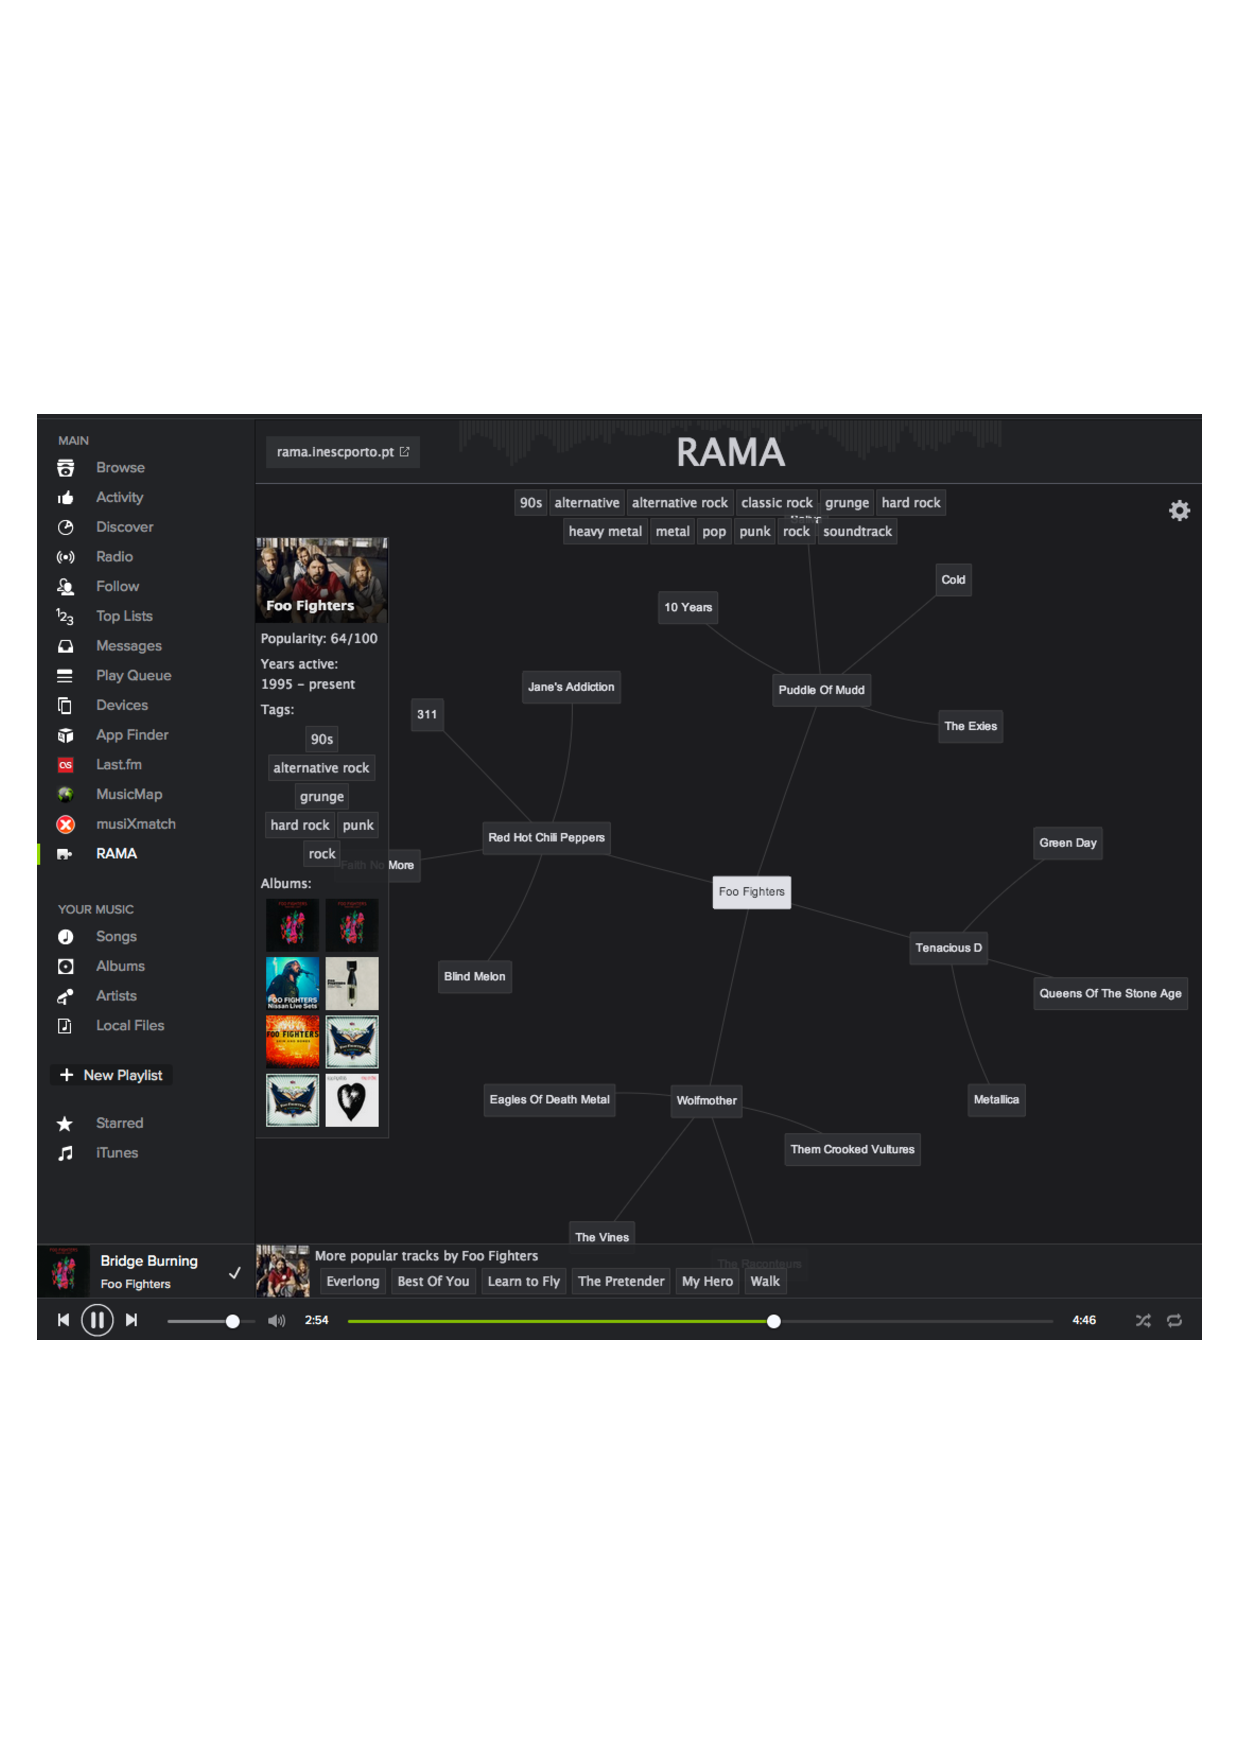
\includegraphics[width=\textwidth]{graph_rootnode.pdf}
        \end{center}
        \caption{The first drawn graph uses the current playing artist (lower left corner) as the root node.}
        \label{fig:graph_rootnode}
      \end{figure}

      The graph-like structure of the map, is created by recursively fetching a list of related artists from each artist. Once a certain pre-established limit of recursive levels is reached, the algorithm stops.

      The map creation algorithm is as follows:

      \lstinputlisting[
        caption={Simplified graph creation algorithm in Javascript (duplicate nodes checking is encapsulated in the insertNode function, as well as duplicate edges in the insertEdge function)}, style=htmlcssjs
      ]
      {snippets/map_creation_alg.js}

      This algorithm, albeit simplified, represents the basic flow when constructing a graph, or more specifically, a tree.
      Since that, in this case of study, the direction of the edges of the graph are not relevant in any way to the artists' map, all of the edges are considered to be undirected.

      Assuming that the insertNode() function only checks for duplicate nodes, i.e., it only inserts unique nodes into the graph, then the resulting graph is one of a tree, since there are no simple cycles in the graph.
      An example of this behaviour can be seen in Figure~\ref{fig:graph_treemode}.

      \begin{figure}[tb]
        \begin{center}
          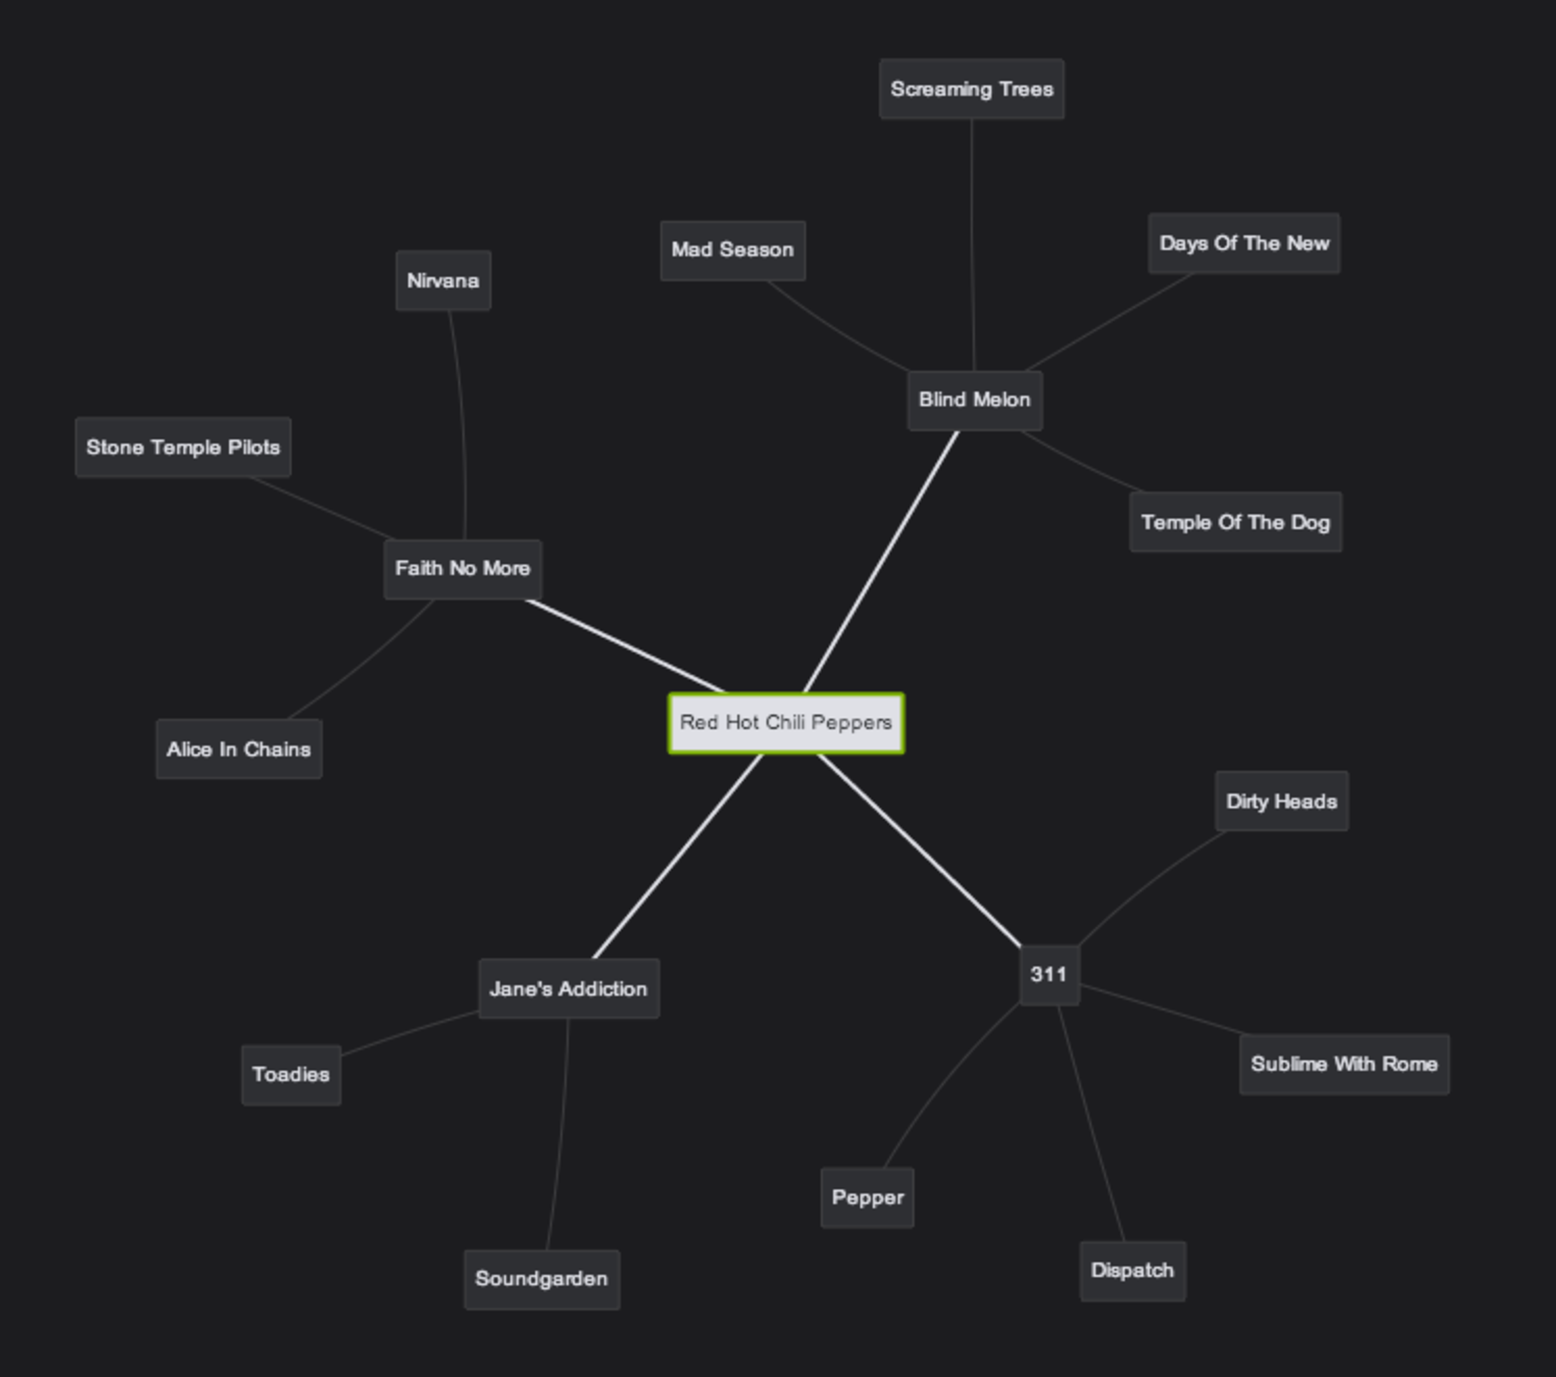
\includegraphics[width=\textwidth]{map_creation_treemode.pdf}
        \end{center}
        \caption{Graph created like a tree with "Red Hot Chilli Peppers" as the root node.}
        \label{fig:graph_treemode}
      \end{figure}

      This approach, however, is not showing all of the available information.
      Given this same example (Figure~\ref{fig:graph_treemode}), the artist node "Stone Temple Pilots" is child of the node artist "Faith No More".
      The algorithm inserted the latter first into the graph.
      After that, when retrieving the childs of "Jane's Addiction", "Stone Templo Pilots" appears, and so the insertNode() function discards the node since it is a duplicate.
      But that means that there is a connection between the both of them that is being discarded.

      To build a graph with all the connections that exist between all of the artists in the graph, the insertNode() function would need to insert the missing edge into the graph by analysing the current graph state.
      An example of this behaviour can be seen in Figure~\ref{fig:graph_notreemode}.

      \begin{figure}[tb]
        \begin{center}
          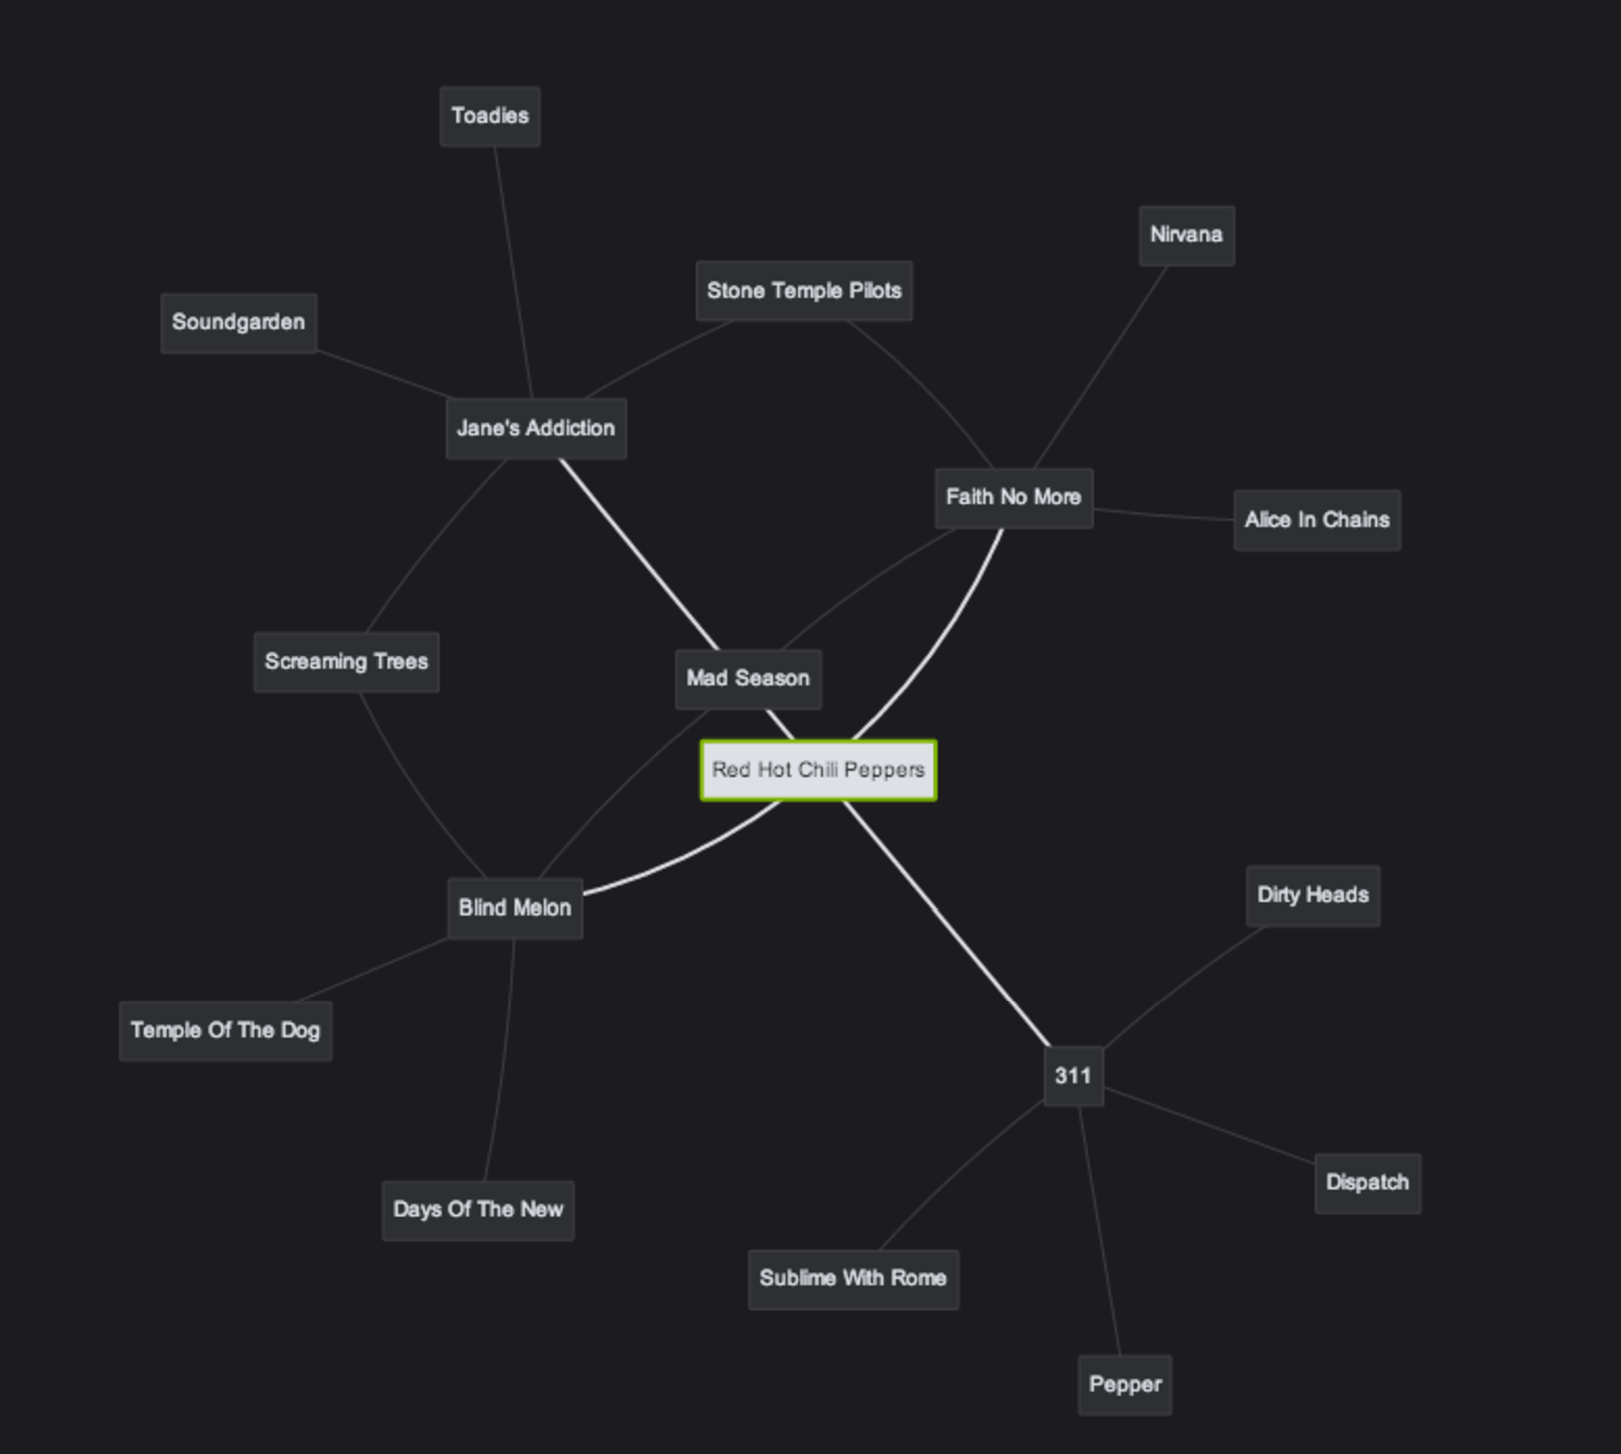
\includegraphics[width=\textwidth]{map_creation_notreemode.pdf}
        \end{center}
        \caption{Graph created with all the connections with "Red Hot Chilli Peppers" as the root node.}
        \label{fig:graph_notreemode}
      \end{figure}



    % subsubsection visualization (end)

    \subsubsection{Graph Edition} % (fold)
      \label{ssub:edition}
    

    % subsubsection edition (end)

    \subsubsection{Tags Overlay} % (fold)
      \label{ssub:tags_overlay}
    


    % subsubsection tags_overlay (end)

    \subsubsection{Artist Info} % (fold)
      \label{ssub:artist_info}
    


    % subsubsection artist_info (end)

  % subsection main_features (end)  


  \subsection{Development Process} % (fold)
    \label{sub:development_process}
  % subsection development_process (end)

% section prototype (end)


\section{Validation} % (fold)
\label{sec:validation}


  \subsection{User Tests} % (fold)
  \label{sub:user_tests}
  
  % subsection user_tests (end)

  \subsection{Data Analysis} % (fold)
  \label{sub:data_analysis}
  
  % subsection data_analysis (end)
% section validation (end)


\section{Conclusions} % (fold)
  \label{sec:conclusions}



% section conclusions (end)